% =============================================================================
% sections/design/rover/navigational_stack.tex  -  Navigational Stack
% Teams: navigation (best guess - unconfirmed) / Status: EXAMPLE (scope approximation)
%
% EXAMPLE CONTENT for scope/layout approximation - not final report text.
% Adapted from the Preliminary Report's "State Estimation and
% Localization" subsection, trimmed to minimal prose. Marked with
% \exampleflag on its heading in the assembler.
%
% Image is a placeholder (teams/navigation/figures/navigational_stack.png)
% - swap it for the real pipeline diagram by overwriting the same file.
% =============================================================================

The rover's localization requirement is an absolute pose error below
\qty{0.8}{\meter} over a \qty{150}{\meter} route. A dual-layered pipeline
meets this in variable lighting and feature-poor environments: a local
Extended Kalman Filter (EKF) fuses visual-inertial and wheel odometry data
for smooth, high-frequency pose estimates, while a global Simultaneous
Localization and Mapping (SLAM) layer corrects drift via scan matching.
ArUco marker detection at known coordinates provides zero-drift absolute
corrections for featureless waypoints. The pipeline is shown in
\autoref{fig:navigational_stack}.

\begin{figure}[!htbp]
    \centering
    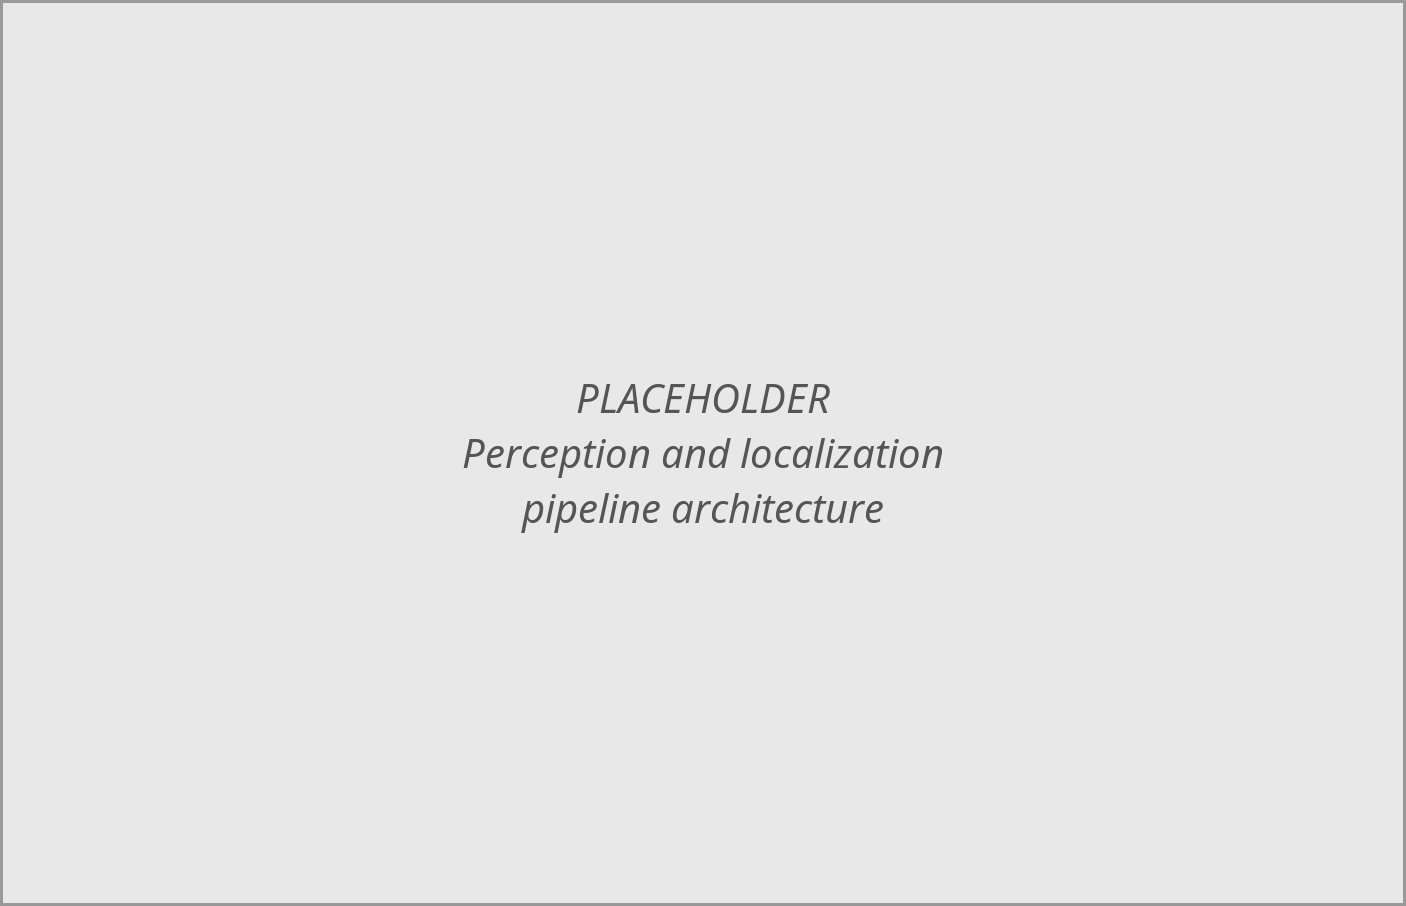
\includegraphics[width=0.85\linewidth]{teams/navigation/figures/navigational_stack}
    \caption{Perception and localization pipeline architecture}
    \label{fig:navigational_stack}
\end{figure}
